\chapter{Desenvolupament}\label{ch:desenvolupament}

En aquest capítol es descriurà el sistema i com són els diferents elements del disseny. Es partirà des de l'estat inicial, explicant la funció de cada part, i després es procedeix a analitzar les mesures que s'han pres per solucionar els problemes detectats. Finalment es descriu com s'han dut a terme aquestes millores.

\section{Estat previ del projecte}\label{sec:punt_de_partida}

Es parteix d'un sistema funcional construït a partir d'una \acsu{PCB}\footnote{Una \ac{PCB} és un suport mecànic sobre le qual es poden soldar diferents dispositius electrònics aprofitant una o diverses capes de coure o algun altre material conductor en les quals s'han gravat les pistes necessàries per connectar els diversos components. Són barates de fabricar i molt més fiables que una placa de proves o \textit{breadboard}.} o placa de circuit imprès\cite{sirio:2015} en forma de \textit{shield} o mòdul d'expansió per a l'\textit{Arduino DUE} (apartat: \ref{subsec:arduino}) modificat per incloure els ajustos necessaris per al seu funcionament bàsic\cite{carles:2017}. Per poder controlar l'espectrofotòmetre s'utilitza un programari fet a mida però poc útil a l'hora de realitzar mesures reals.

Aquest sistema es pot dividir en dos circuits: un responsable de generar el senyal lumínic que emetran els \acp{LED} i un altre que capti aquest senyal i l'interpreti per obtenir informació sobre el medi que es troba entre els \acp{LED} i el fotodíode (apartat: \ref{subsec:diode}). Ambdós circuits estan connectats a l'\hyperref[subsec:arduino]{\textit{Arduino}} per poder comunicar-se amb l'ordinador i s'han inclòs a la \ac{PCB}.

\begin{figure}[htp]
	\centering
	\includegraphics[width=0.7\textwidth]{Figures/esquema_sistema.pdf}
	\caption[Esquema general del sistema]{\textit{Esquema general del sistema}\\{\footnotesize L'\textit{Arduino DUE} actua com a centre neuràlgic per comunicar tots els components del sistema. L'ordinador només serveix com a centre de control i recepció de dades. La \ac{PCB} conté tot el circuit necessari per poder mesurar la contaminació.}}
	\label{fig:esquema_sistema}
\end{figure}

\subsection{Senyal}

Treballar amb \acp{LED} implica que no es pot aconseguir una ona coherent i, per tant, es necessita trobar una manera alternativa de diferenciar el senyal de la llum ambiental. Si es modifica la intensitat lumínica sinusoïdalment, es pot idear un mètode per aïllar molt fàcilment el senyal desitjat. S'ha decidit utilitzar una freqüència de \SI{7}{\kilo\hertz} fixada digitalment per l'\hyperref[subsec:arduino]{\textit{Arduino}}.

Des de l'ordinador es pot configurar tant l'amplitud com l'\textit{offset} de l'ona, juntament amb el color del \ac{LED} que s'activarà. Poder ajustar l'\textit{offset} permetrà situar l'amplitud de treball en la zona de comportament lineal dels \acp{LED}.

\subsection{Circuit generador del senyal}\label{subsec:circuit_generador}

Aquest circuit és el responsable de transformar el senyal sinusoïdal de la sortida del convertidor digital a analògic (\ac{DAC}) en un senyal lumínic amb la mateixa forma i característiques equivalents. En la figura \ref{fig:esquema_circuit_generador} es pot veure l'esquema simplificat d'aquest circuit.

\begin{figure}[htp]
	\centering
	\includegraphics[width=0.8\textwidth]{Figures/esquema_circuit_generador.pdf}
	\caption[Esquema del circuit generador del senyal]{\textit{Esquema del circuit generador del senyal}}
	\label{fig:esquema_circuit_generador}
\end{figure}

\subsubsection{\acs{DAC} de l'\hyperref[subsec:arduino]{\textit{Arduino}}}

Tradueix una seqüència digital de \textit{bytes} a un senyal analògic. En el cas de l'\textit{Arudino DUE}, té una resolució de fins a \num{12} bits\footnote{Una resolució de \num{12} bits equival a \num{4096} nivells entre el màxim i el mínim de tensió que el \ac{DAC} és capaç de subministrar.} i pot subministrar un senyal d'entre \SIrange[range-phrase = \ i\ ]{0.55}{2.75}{\volt} de tensió. Un dels problemes que es van detectar als inicis del projecte és que calia ajustar aquest senyal al rang dinàmic mitjançant un amplificador.

\subsubsection{Amplificador del senyal}

Els \acp{OPAMP} \textit{rail-to-rail} utilitzats (apartat: \ref{subsec:amplificador_operacioanl}) tenen un rang dinàmic de \SIrange[range-phrase = \ a\ ]{0}{5}{\volt} ja que la màxima tensió que pot subministrar l'Arduino és $ \acs{VCC} = \SI{5}{\volt} $ i l'alimentació negativa dels \acp{OPAMP} està connectada a terra. Això implica que cal ajustar el màxim del senyal a la sortida de l'amplificador a aquests \SI{5}{\volt}. 

Un altre punt a tenir en compte és que els díodes (i per extensió els \acp{LED}) necessiten una mínima diferència de tensió per a emetre llum, en la majoria de casos per sobre dels \SI{0.55}{\volt} mínims que subministra el \ac{DAC}. L'amplificador del senyal també s'encarrega d'augmentar aquest mínim per sobre de \SI{1.4}{\volt} aprofitant el circuit de la figura \ref{fig:schematic_amplificador}.

\begin{figure}[htp]
	\centering
	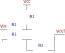
\includegraphics[width=0.5\textwidth]{Figures/schematic_amplificador.pdf}
	\caption[Amplificador del senyal]{Schematic\textit{ de l'amplificador del senyal}\\{\footnotesize Les resistències utilitzades són $ \acs{R}_1=\SI{16.4}{\kilo\ohm} $, $ \acs{R}_2 = \acs{R}_4 =\SI{1}{\kilo\ohm} $ i $ \acs{R}_3=\SI{1.3}{\kilo\ohm} $. L'\ac{OPAMP} és necessari que sigui \textit{rail-to-rail} per garantir el màxim rang dinàmic.}}
	\label{fig:schematic_amplificador}
\end{figure}

Si s'analitza aquest circuit en detall es pot calcular el rang que tindrà la tensió de sortida (\acsu{VOUT}) en funció del rang de la tensió d'entrada (\acsu{VIN}), que no és cap altre que la sortida del \ac{DAC}\footnote{Les resistències escollides no són les ideals degut a que no es volia utilitzar moltes resistències petites per assolir el valor esperat al resoldre les equacions.}:

\begin{multline}
\acs{VOUT} = \left(1 + \frac{\acs{R}_4}{\acs{R}_3}\right) \left(\frac{\acs{VCC}\cdot \acs{R}_2}{\acs{R}_1 + \acs{R}_2} + \frac{\acs{R}_1}{\acs{R}_1 + \acs{R}_2} \acs{VIN}\right) =\\=\left(1 + \frac{\SI{1}{\kilo\ohm}}{\SI{1.3}{\kilo\ohm}}\right) \left(\frac{\SI{5}{\volt}\cdot \SI{1}{\kilo\ohm}}{\SI{16.4}{\kilo\ohm} + \SI{1}{\kilo\ohm}} + \frac{\SI{16.4}{\kilo\ohm}}{\SI{16.4}{\kilo\ohm} + \SI{1}{\kilo\ohm}} \acs{VIN}\right)
\end{multline}

\begin{equation}
\acs{VOUT} = \left[\SIrange[range-phrase = \ -\ ]{1.4}{5.1}{\volt}\right]
\end{equation}

\subsubsection{Font de corrent}

Els \acp{LED} s'alimenten amb corrent però l'\hyperref[subsec:arduino]{\textit{Arduino}} només pot subministrar un senyal de tensió. Així doncs cal utilitzar una font de corrent com la que es pot observar en la figura \ref{fig:schematic_font_corrent}. El corrent generat ve determinat directament per la tensió que surt de l'amplificador del senyal (eq. \ref{eq:font_tensio}).

\begin{figure}[htp]
	\centering
	\includegraphics[width=0.4\textwidth]{Figures/schematic_font_corrent.pdf}
	\caption[Font de corrent]{Schematic\textit{ de la font de corrent}}
	\label{fig:schematic_font_corrent}
\end{figure}

\begin{equation}\label{eq:font_tensio}
\acs{I}_{\acs{LED}}=\frac{\acs{VCC}-\acs{VIN}}{\acs{R}}
\end{equation}

\subsubsection{Díodes \ac{LED} \acsu{RGB}}

 El conjunt de \acp{LED} originalment plantejat havia de ser realment \ac{RGB} (tres díodes en un sol dispositiu) per poder avaluar un ampli rang de longituds d'ona. Malauradament va resultar que la lluminositat del \ac{LED} blau no era suficient i impedia realitzar mesures significatives. Així doncs es va decidir canviar, encara que fos temporalment, el díode blau per un de taronja mitjançant un xip diferent que incorporés els tres colors resultants. Ambdós models comparteixen el mateix funcionament: tenen un càtode comú connectat a la font de corrent i cada ànode es comunica amb una sortida digital diferent de l'\hyperref[subsec:arduino]{\textit{Arduino}}. Sempre que un ànode determinat estigui connectat al terra per mitjà d'aquestes sortides digitals, el \ac{LED} s'i\lgem uminarà.
 
\subsubsection{Sortides digitals de l'\hyperref[subsec:arduino]{\textit{Arduino}} i \textit{switch array}}

Per controlar quin \ac{LED} està actiu en tot moment no n'hi ha prou amb connectar els díodes directament a les sortides digitals de l'\hyperref[subsec:arduino]{\textit{Arduino}}. Cal introduir un dispositiu de seguretat que eviti valors elevats de corrent per protegir tant l'\hyperref[subsec:arduino]{\textit{Arduino}} com els \acp{LED}. És per això que s'introdueix un \textit{switch array} que no només compleix aquesta funció sinó que inverteix el valor de les sortides digitals per facilitar la creació del software\footnote{Per connectar els ànodes dels \acp{LED} a terra (i així encendre'ls) es necessitaria un \num{0} de sortida digital, deixant en \num{1} les altres sortides pels díodes que es volen mantenir apagats. Amb la introducció dels inversors del \textit{switch array} es pot associar l'\num{1} a encès i el \num{0} a apagat, clarificant  així el funcionament del sistema per als programadors.}.

\subsection{Circuit receptor i de processament del senyal}\label{subsec:circuit_receptor}

Aquest circuit és responsable de captar el senyal lumínic dels \acp{LED} i transformar-lo en un valor de tensió dins dels límits de l'\ac{ADC} que equivalgui a la transmitància del medi comprés entre els \acp{LED} i el fotodíode (apartat: \ref{subsec:lambert-beer}). En la figura \ref{fig:esquema_circuit_receptor_1} es pot veure l'esquema simplificat d'aquests circuit.

\begin{figure}[htp]
	\centering
	\includegraphics[width=0.8\textwidth]{Figures/esquema_circuit_receptor_1.pdf}
	\caption[Esquema del circuit receptor i de processament del senyal]{\textit{Esquema del circuit receptor i de processament del senyal}\\{\footnotesize S'indica on va co\lgem ocat el circuit que controla el guany variable.}}
	\label{fig:esquema_circuit_receptor_1}
\end{figure}

\subsubsection{Fotodíode}

D'una manera similar al que va passar amb el \ac{LED} blau, inicialment es va decidir utilitzar un fototransistor per captar el senyal lumínic però es va haver de descartar ja que li faltava precisió per detectar el sinus. L'alternativa per la qual es va optar és el fotodíode (apartat: \ref{subsec:diode}) que tradueix la intensitat de llum que rep en un senyal de corrent, en aquest cas sinusoïdal, però incorporant quantitats importants de soroll ambiental.

\subsubsection{\acl{TIA} i cance\lgem ador de contínua}\label{itm:vref}

Com que el fotodíode només és capaç de subministrar un senyal de corrent, cal primer transformar-lo en voltatge ja que, sinó, no es podrà filtrar ni treballar amb ella per obtenir un valor que accepti l'\ac{ADC}. És per això que s'utilitza un amplificador de transimpedància (\acs{TIA}) just després del fotodíode.

Tot i així, cal tenir en compte que el fotodíode no només detecta el senyal dels \acp{LED}. De fet, la principal font de llum és l'ambiental i això implica que, si simplement s'utilitza un \ac{TIA}, l'\ac{OPAMP} es saturarà i no es podrà treballar amb el senyal. Cal doncs introduir algun sistema que cance\lgem i l'\textit{offset} del fotodíode i deixi només el sinus.

Una solució passa per utilitzar un circuit integrador no-inversor que retorna un corrent equivalent a la integral en el temps de tots els senyals per sota d'una determinada freqüència. Si s'aconsegueix fer que aquest  corrent s'oposi al produït pel fotodíode es podrà cance\lgem ar el senyal continu. Es pot trobar més informació sobre el \ac{TIA} i el circuit integrador no-inversor a l'apartat \ref{subsec:amplificador_operacioanl}.

A tot plegat, s'introdueix un altre punt a tenir en compte: el senyal sinusoïdal necessita un mínim \textit{offset} equivalent a l'amplitud d'aquest per a què els \acp{OPAMP} no el retallin per sota de \SI{0}{\volt}\footnote{El rang dinàmic dels \acp{OPAMP} en el circuit utilitzat és de \SIrange[range-phrase = \ a\ ]{0}{5}{\volt}.}. Per solucionar-ho es referencien tant el \ac{TIA} com el cance\lgem ador de contínua a $ \acsu{VREF} = \SI{2.5}{\volt} $, just al mig del rang dinàmic. Aquests \SI{2.5}{\volt} s'aconsegueixen mitjançant un divisor de tensió (apartat: \ref{subsec:divisor_tensio}) i s'hauran d'introduir com a \ac{VREF} en tots els \acp{OPAMP} que treballin amb el senyal sinusoïdal.

Es pot veure la disposició tant del \ac{TIA} com del cance\lgem ador de contínua juntament amb el fotodíode en la figura \ref{fig:schematic_tia}. S'han escollit els valors dels resistors i condensadors per aconseguir una freqüència de tall (\acsu{FC})  inferior als \SI{7}{\kilo\hertz} del senyal sinusoïdal:

\begin{figure}[htp]
	\centering
	\includegraphics[width=0.5\textwidth]{Figures/schematic_tia.pdf}
	\caption[\acs{TIA} i cance\lgem ador de contínua]{Schematic\textit{ del \ac{TIA} i del cance\lgem ador de contínua}\\{\footnotesize Els components utilitzats són $ \acs{C}_1 = \acs{C}_2=\SI{1}{\micro\farad} $, $ \acs{R}_1 = \acs{R}_3 =\SI{10}{\kilo\ohm} $, $ \acs{R}_2=\SI{10}{\kilo\ohm} $ i $ \acs{R}_4=\SI{330}{\ohm} $.}}
	\label{fig:schematic_tia}
\end{figure}

\begin{equation}
\acs{FC} = \frac{\acs{R}_4}{2\pi \acs{R}_1 \acs{R}_2 \acs{C}_1} = \frac{\SI{330}{\ohm}}{2\pi \cdot \SI{10e3}{\ohm} \cdot \SI{10e3}{\ohm} \cdot \SI{1e-6}{\farad}} = \SI{0.53}{\hertz}
\end{equation}

El valor de la resistència $ \acs{R}_2 $ també determina el corrent màxim (\acsu{IMAX}) que es pot cancel·lar. En els experiments realitzats s'ha determinat que aquests \SI{0.25}{\milli\ampere} són suficients per cance\lgem ar qualsevol font de llum ambiental.

\begin{equation}
\acs{IMAX} = \frac{\acs{VREF}}{\acs{R}_2} = \frac{\SI{2.5}{\volt}}{\SI{10}{\kilo\ohm}} = \SI{0.25}{\milli\ampere}
\end{equation}

\subsubsection{Filtre passa-banda}

La sortida del \ac{TIA} està força neta de senyals amb freqüències per sota de \SI{7}{\kilo\hertz} (malgrat tenir encara algunes traces degut a que $ \ac{FC} = \SI{0.53}{\kilo\hertz} $), però té força soroll amb freqüències superiors a el senyal sinusoïdal que cal aïllar.

S'ha optat per utilitzar dos filtres \textit{biquad} passa-banda \textit{Sallen-Key} (apartat: \ref{subsec:amplificador_operacioanl}) en cascada per cance\lgem ar totes les freqüències que no es corresponguin a la seleccionada.

Es pot trobar un \textit{schematic} amb l'estructura de cada filtre a la figura \ref{fig:schematic_filtre_p-banda} juntament amb els càlculs per trobar-ne el guany intern ($ \acsu{H}_0 $), \ac{Q}, \ac{F0} i \ac{AB}. Cal destacar que l'\ac{OPAMP} s'ha hagut de referenciar amb \ac{VREF} tal com s'ha comentat en l'\hyperref[itm:vref]{apartat anterior}.

\begin{figure}[htp]
	\centering
	\includegraphics[width=0.5\textwidth]{Figures/schematic_filtre_p-banda.pdf}
	\caption[Filtre passa-banda]{Schematic\textit{ del filtre passa-banda}\\{\footnotesize Els components utilitzats són $ \acs{C}_1 = \acs{C}_2=\SI{10}{\nano\farad} $, $ \acs{R}_1 = \SI{16}{\kilo\ohm} $, $ \acs{R}_2 = \SI{120}{\ohm} $ i $ \acs{R}_3=\SI{40}{\kilo\ohm} $.}}
	\label{fig:schematic_filtre_p-banda}
\end{figure}

\begin{equation}
\acs{H}_0 = \frac{\acs{R}_3}{2\acs{R}_1} = \frac{\SI{40}{\kilo\ohm}}{2\cdot\SI{16}{\kilo\ohm}} = \num{1.25}
\end{equation}

\begin{multline}
\acs{Q} = \frac{\sqrt{\num{2}}}{\num{4}}\sqrt{\frac{\acs{R}_3+\sqrt{8\acs{H}_0\acs{R}_2^2+\acs{R}_3^2}}{\acs{R}_2}} =\\= \frac{\sqrt{\num{2}}}{\num{4}}\sqrt{\frac{\SI{40e3}{\ohm}+\sqrt{8\cdot\num{1.25}(\SI{120}{\ohm})^2+(\SI{40e3}{\ohm})^2}}{\SI{120}{\ohm}}} = \num{9.13}
\end{multline}

\begin{equation}
\acs{F0} = \frac{\acs{Q}}{\pi \acs{R}_3\acs{C}_1} = \frac{\num{9.13}}{\pi\cdot\SI{40e3}{\ohm}\cdot\SI{10e-9}{\farad}} = \SI{7.27e3}{\hertz} = \SI{7.27}{\kilo\hertz}
\end{equation}

\begin{equation}
\acs{AB} = \frac{\acs{F0}}{\acs{Q}} = \frac{\SI{7.27e3}{\hertz}}{\num{9.13}} = \SI{796}{\hertz}
\end{equation}

El fet que $ \ac{H}_0 > \num{1} $ permet que el senyal sinusoïdal de \SI{7}{\kilo\hertz} no sigui atenuat per aquests filtres que no estan perfectament ajustats a aquesta freqüència central.

\subsubsection{Detector d'envolupant}

Un detector d'envolupant no és res més que un circuit rectificador de mitja ona (apartat: \ref{subsec:circuit_rectificador}) que retorna el punt màxim dels pics de l'ona sinusoïdal. S'utilitza un díode \textit{Schottky} que té un \ac{VT} petit, però no nul\footnote{Un dels objectius d'aquest projecte és solucionar justament els problemes que comporta que $ \ac{VT} \neq 0 $.}, connectat en sèrie a un circuit \ac{RC} (fig. \ref{fig:schematic_rectificador_1}).

\begin{figure}[htp]
	\centering
	\includegraphics[width=0.3\textwidth]{Figures/schematic_rectificador_1.pdf}
	\caption[Circuit rectificador]{Schematic\textit{ del circuit rectificador}\\{\footnotesize Els components utilitzats són $ \acs{R} = \SI{10}{\kilo\ohm} $ i $ \acs{C} = \SI{220}{\nano\farad} $.}}
	\label{fig:schematic_rectificador_1}
\end{figure}

La constant de temps ($ \acs{R}\cdot\acs{C} $) d'aquest rectificador ha de ser superior al període del senyal que es vol analitzar i es pot comprovar mitjançant es equacions \ref{eq:rc1} i \ref{eq:rc2}.

\begin{equation}\label{eq:rc1}
\acs{R}\acs{C} > \frac{\num{1}}{\ac{F0}} \Longrightarrow  \SI{10e3}{\ohm}\cdot\SI{220e-9}{\farad} > \frac{\num{1}}{\SI{7e3}{\hertz}}
\end{equation}

\begin{equation}\label{eq:rc2}
\SI{2.2e-3}{\second} > \SI{1.4e-4}{\second}
\end{equation}

Com que el senyal ja ha estat molt filtrat, no és necessari ajustar excessivament la constant de temps i creix en importància el fet de no utilitzar resistors o condensadors grans que puguin introduir soroll no desitjat.

\subsubsection{Filtre restador passa-baix}

Els rectificadors no donen un senyal net sense soroll, \ac{VOUT} té més aviat una forma de serra (considerant que \ac{VIN} és sinusoïdal). Així doncs, cal tornar a filtrar ja que l'objectiu és obtenir un senyal pla, és a dir amb una freqüència tendint a zero ($ \acsu{F} \rightarrow \num{0} $). Es tornaran a utilitzar dos filtres \textit{biquad} \textit{Sallen-Key}, aquest cop passa-baix (apartat: \ref{subsec:amplificador_operacioanl}), en sèrie per maximitzar la capacitat de filtratge.

A més, cal tenir en compte que el senyal sinusoïdal tenia un \textit{offset} de \SI{2.5}{\volt} que ara resulta només en una pèrdua de rang dinàmic. L'\ac{ADC} només accepta tensions de \SIrange[range-phrase = \ a\ ]{0}{3.3}{\volt} i aquests filtres són els últims components previs a la lectura de l'\hyperref[subsec:arduino]{\textit{Arduino}}. Es poden aprofitar els dos filtres per restar aquest \textit{offset} en dues etapes i a la vegada introduir un cert guany que ajusti la tensió màxima (\acsu{VMAX}) a aquests \SI{3.3}{\volt}.

Es pot trobar un \textit{schematic} amb l'estructura de cada filtre a la figura \ref{fig:schematic_filtre_p-baix} juntament amb els càlculs per trobar-ne \ac{FC}, $ \ac{H}_0 $, \ac{Q} i \ac{AB}.

\begin{figure}[htp]
	\centering
	\includegraphics[width=0.5\textwidth]{Figures/schematic_filtre_p-baix.pdf}
	\caption[Filtre passa-baix]{Schematic\textit{ del filtre passa-baix}\\{\footnotesize Els components utilitzats són $ \acs{C}_1 = \acs{C}_2 = \SI{1.5}{\micro\farad} $, $ \acs{R}_1 = \SI{3}{\kilo\ohm} $, $ \acs{R}_2 = \acs{R}_3 = \SI{1}{\kilo\ohm} $, $ \acs{R}_4 = \acs{R}_5 = \SI{3.6}{\kilo\ohm} $.}}
	\label{fig:schematic_filtre_p-baix}
\end{figure}

\begin{equation}
\acs{FC} = \frac{\num{1}}{\num{2}\pi\acs{R}_4\acs{C}_1} = \frac{\num{1}}{\num{2}\pi\cdot\SI{3.6e3}{\ohm}\cdot\SI{1.5e-6}{\farad}} = \SI{29}{\hertz}
\end{equation}

\begin{equation}
\acs{H}_0 = \num{1} + \acs{R}_3\left(\frac{\num{1}}{\acs{R}_2} + \frac{\num{1}}{\acs{R}_1}\right) = \num{1} + \SI{1}{\kilo\ohm}\left(\frac{\num{1}}{\SI{1}{\kilo\ohm}} + \frac{\num{1}}{\SI{3}{\kilo\ohm}}\right) = \num{2.3}
\end{equation}

\begin{equation}
\acs{Q} = \frac{\num{1}}{\num{3} - \acs{H}_0} = \frac{\num{1}}{\num{3} - \num{2.3}} = \num{1.5}
\end{equation}

\begin{equation}
\acs{AB} = \frac{\acs{FC}}{\acs{Q}} = \frac{\SI{29}{\hertz}}{\num{1.5}} = \SI{19}{\hertz}
\end{equation}

Així doncs, les freqüències superiors a \SI{19}{\hertz} seran àmpliament cance\lgem ades deixant una quantitat marginal de soroll. Es podria reduir aquest valor de \ac{AB} augmentant el valor de $ \acs{R}_4 $ i $ \acs{R}_5 $ (sempre mantenint-los igual) però llavors s'introduiria més soroll al sistema provinent, aquest cop, dels resistors mateixos.

\subsubsection{\acs{ADC} de l'\hyperref[subsec:arduino]{\textit{Arduino}}}

El senyal ja està a punt per enviat a l'\ac{ADC} de l'\hyperref[subsec:arduino]{\textit{Arduino}} però, per evitar cremar la placa, s'ha optat per introduir un sistema de seguretat mitjançant la sortida de \SI{3.3}{\volt} que proporciona la mateixa \hyperref[subsec:arduino]{\textit{Arduino}} i un díode tal com es mostra a la figura \ref{fig:schematic_adc}:

\begin{figure}[htp]
	\centering
	\includegraphics[width=0.25\textwidth]{Figures/schematic_adc.pdf}
	\caption[Circuit de seguretat per l'\acs{ADC}]{Schematic\textit{ del circuit de seguretat per l'\ac{ADC}}\\{\footnotesize El resistor utilitzat és de \SI{1}{\kilo\ohm}.}}
	\label{fig:schematic_adc}
\end{figure}

L'\ac{ADC} tradueix senyals analògics a una seqüència digital de \textit{bytes}. Accepta tensions d'entrada d'entre \SIrange[range-phrase = \ i\ ]{0}{3.3}{\volt} i té una resolució de \num{12} bits.

\section{Millores del circuit electrònic}\label{sec:millores_del_circuit_electronic}

Un dels punts a considerats per millorar és la introducció d'una manera de controlar el guany del circuit per poder ajustar el màxim del senyal al rang dinàmic de l'\ac{ADC}. Es va proposar utilitzar un circuit multiplicador que es podria controlar amb el segon \ac{DAC} de l'\hyperref[subsec:arduino]{\textit{Arduino}} i així poder-hi accedir des del programari de control.

A més, com ja s'ha comentat en l'apartat \ref{subsec:circuit_receptor}, un altre punt que es podria millorar és el rectificador del detector d'envolupant, que limita significativament el rang dinàmic degut a que conté un díode amb \ac{VT} no nul. Es pot millorar utilitzant un super-díode que permeti aconseguir un rectificador sense pèrdues.

\subsection{Circuit multiplicador}\label{subsec:circuit_multiplicador}

Un circuit multiplicador convencional consta de quatre \acp{OPAMP}. Com que només es necessita multiplicar el senyal per una constant, no és necessari utilitzar els quatre i es pot prescindir de l'amplificador que s'encarregaria d'aplicar la funció logarítmica a la tensió provinent del segon \ac{DAC} de l'\hyperref[subsec:arduino]{\textit{Arduino}}.

Sacrificar aquest \ac{OPAMP} només implica que la resposta del circuit multiplicador no serà lineal, però això es pot solucionar fàcilment amb el \textit{software} que controla el sistema.

Així doncs, el circuit de tres \acp{OPAMP} haurà d'aplicar en primer lloc una funció logarítmica al senyal, sumar-li el voltatge del segon \ac{DAC} i, finalment, aplicar-li una funció exponencial (fig. \ref{fig:schematic_multiplicador}).

\begin{figure}[htp]
	\centering
	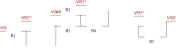
\includegraphics[width=0.8\textwidth]{Figures/schematic_multiplicador.pdf}
	\caption[Circuit multiplicador final]{Schematic\textit{ del circuit multiplicador final}\\{\footnotesize Els resistors utilitzats són $ \acs{R}_1 = \acs{R}_5 = \SI{10.1}{\kilo\ohm} $, $ \acs{R}_2 = \SI{5.6}{\kilo\ohm} $, $ \acs{R}_3 = \acs{R}_4 = \SI{1}{\kilo\ohm} $.}}
	\label{fig:schematic_multiplicador}
\end{figure}

Aquests \acp{OPAMP} també cal referenciar-los, però no es pot fer de la mateixa manera que en la resta. En aquests, la \ac{VREF} ha d'estar lleugerament per sota del valor que s'utilitza en els altres per al correcte funcionament dels amplificadors logarítmics. S'ha decidit posar la referència a \SI{2.4}{\volt} i per obtenir-los s'ha aprofitat el divisor de tensió que ja s'utilitzava per obtenir els \SI{2.5}{\volt} anteriors i se li ha afegit una segona divisió després de la primera.

El fet d'utilitzar dos díodes en sèrie enlloc de només un accentua el caràcter logarítmic o exponencial  dels dos \acp{OPAMP} terminals.

\subsection{Rectificador}\label{subsec:rectificador}

Substituir un díode per un super-díode implica poca modificació del circuit original i només es necessita tenir un \ac{OPAMP} lliure per poder aprofitar-lo. En la figura \ref{fig:schematic_rectificador_2} es pot veure com l'única diferència és la introducció de l'\ac{OPAMP} retroalimentat negativament mitjançant un díode en la mateixa posició on originalment hi havia aquest component que es volia substituir (fig. \ref{fig:schematic_rectificador_1}).

\begin{figure}[htp]
	\centering
	\includegraphics[width=0.3\textwidth]{Figures/schematic_rectificador_2.pdf}
	\caption[Circuit rectificador amb un súper-díode]{Schematic\textit{ del circuit rectificador amb un súper-díode}\\{\footnotesize Els components utilitzats són $ \acs{R} = \SI{10}{\kilo\ohm} $ i $ \acs{C} = \SI{220}{\nano\farad} $.}}
	\label{fig:schematic_rectificador_2}
\end{figure}

\begin{figure}[htp]
	\centering
	\includegraphics[width=0.8\textwidth]{Figures/esquema_circuit_receptor_2.pdf}
	\caption[Esquema del circuit receptor i de processament del senyal després de les millores]{\textit{Esquema del circuit receptor i de processament del senyal després de les millores}\\{\footnotesize El guany variable ja està introduït al sistema, juntament amb el super-díode del detector d'envolupant.}}
	\label{fig:esquema_circuit_receptor_2}
\end{figure}

\section{Disseny i soldatge de la \ac{PCB}}\label{sec:disseny_i_soldatge_pcb}

La part electrònica d'aquest projecte ha estat modificada notablement i cal fabricar una \ac{PCB} que incorpori totes les millores introduïdes.

\subsection{Dibuix de l'\textit{schematic}}\label{subsec:schematic}

S'ha utilitzat el programa \textit{Allegro Design Entry CIS} per dibuixar l'\textit{schematic} ja que forma part del paquet professional de software per al desenvolupament de \acp{PCB} del qual es disposa llicència en l'\ac{IMB}-\ac{CNM} - \ac{CSIC}. Es tracta d'un programa molt complet i que està íntimament relacionat amb el que s'utilitzarà per a dibuixar la \ac{PCB} i generar els fitxers GERBER. A més, el el mateix programa que s'ha utilitzat per realitzar simulacions sobre moltes parts del circuit abans de muntar-les a la placa de proves.

Es va optar per un disseny de l'\textit{schematic} jeràrquic, és a dir: es treballa per blocs interconnectats entre sí. Cada bloc pot contenir més blocs que generen un altre nivell jeràrquic, i així successivament fins arribar als components més bàsics. Aquesta manera de treballar permet una fàcil comprensió del funcionament del circuit sense necessitar una anàlisi extensa de les connexions establertes.

Pel cas del present sistema s'ha decidit dividir el circuit en quatre blocs bàsics que es corresponen a:

\begin{itemize}
	
	\item{\textbf{\hyperref[subsec:arduino]{\textit{Arduino DUE}}}: }Conté tots els elements relacionats amb l'\hyperref[subsec:arduino]{\textit{Arduino}} i com es connecta amb la resta del circuit.
	
	\item{\textbf{Administració de les fonts de tensió}: }S'hi detalla com s'obtenen els voltatges de referència de \SI{2.4}{\volt} i \SI{2.5}{\volt}, juntament amb els dispositius relacionats amb la seguretat dels components del circuit.
	
	\item{\textbf{Circuit generador del senyal}: }Conté el circuit explicat en l'apartat \ref{subsec:circuit_generador}.
	
	\item{\textbf{Circuit receptor i de processament del senyal}: }Conté el circuit explicat en l'apartat \ref{subsec:circuit_receptor}, juntament amb el circuit multiplicador (apartat: \ref{subsec:circuit_multiplicador}) i el rectificador (apartat: \ref{subsec:rectificador}).
	
\end{itemize}

\begin{figure}[htp]
	\centering
	\includegraphics[width=0.8\textwidth]{Figures/schematic.png}
	\caption[\textit{Schematic} realitzat amb l'\textit{Allegro Design Entry CIS}]{Schematic\textit{ realitzat amb l'}Allegro Design Entry CIS\\{\footnotesize Es poden observar com estan distribuïts els quatre blocs.}}
	\label{fig:schematic}
\end{figure}

\subsection{Dibuix de la \acs{PCB} i generació dels fitxers \textit{GERBER}}\label{subsec:gerbers}

Com ja s'ha comentat en l'\hyperref[subsec:schematic]{\textit{apartat anterior}}, s'ha decidit utilitzar un programa molt lligat a l'\textit{Allegro Design Entry CIS} per al dibuix de la \ac{PCB} anomenat \textit{Allegro \ac{PCB} Editor}. Aquest programa et permet ajustar tots els paràmetres corresponents a les limitacions de la màquina de \ac{CNC}.

És necessari assignar prèviament una empremta a cada component de l'\textit{schematic} i així el programa només necessitarà que se li digui on co\lgem ocar cada element i per on haurien de passar les pistes. De fet, es podria demanar al mateix programa que calculés per on haurien de passar les pistes, però per a un circuit d'aquestes dimensions és contraproduent.

Els fitxers \textit{GERBER} són els que la màquina \ac{CNC} podrà llegir i hi cal especificar les dimensions de la placa, on s'han de fer forats (per co\lgem ocar-hi segons quins components o per comunicar les diferents capes de la \ac{PCB}) i quin dibuix s'ha de gravar a les làmines de coure que formaran cada capa.

%\begin{figure}[!ht]
%	\centering
%	\includegraphics[width=0.8\textwidth]{Figures/pcb_top_white.png}
%	
%	(a) Capa superior o \textit{top}.
%	
%	\includegraphics[width=0.8\textwidth]{Figures/pcb_bottom_white.png}
%	
%	(b) Capa inferior o \textit{bottom}.
%	
%	\caption[Disseny de la \acs{PCB}]{\textit{Disseny de la \acs{PCB}}\\{\footnotesize Es poden observar les dues capes utilitzades amb colors diferents: verd per la capa superior o \textit{top} (a) i groc per la capa inferior o \textit{bottom} (b). Aquests dissenys han estat realitzats amb el programa \textit{Allegro \ac{PCB} Editor}.}}
%	\label{fig:pcb}
%\end{figure}

\begin{figure}[ht]
\begin{tabular}{c}
	\begin{tabular}{cc}
		\includegraphics[width=0.45\textwidth]{Figures/pcb_top_white.png} & \includegraphics[width=0.45\textwidth]{Figures/pcb_top.png} \\ 
	\end{tabular}  \\ 
	(a) Capa superior o \textit{top} \\ 
	\begin{tabular}{cc}
		\includegraphics[width=0.45\textwidth]{Figures/pcb_bottom_white.png} & \includegraphics[width=0.45\textwidth]{Figures/pcb_bottom.png} \\ 
	\end{tabular}  \\ 
	(b) Capa inferior o \textit{bottom} \\ 
\end{tabular} 
\caption[Disseny de la \acs{PCB}]{\textit{Disseny de la \acs{PCB}}\\{\footnotesize Es poden observar les dues capes utilitzades amb colors diferents: verd per la capa superior o \textit{top} (a) i groc per la capa inferior o \textit{bottom} (b). A la dreta es pot observar el resultat final abans de soldar. Aquests dissenys han estat realitzats amb el programa \textit{Allegro \ac{PCB} Editor}.}}
\label{fig:pcb}
\end{figure}

\section{Programari de control}\label{sec:descripcio_del_sistema}

El programari de control original constava de principalment dues parts: el \textit{firmware} de l'\hyperref[subsec:arduino]{\textit{Arduino}} escrit en \textit{C++}\footnote{El \textit{C++} és un llenguatge orientat a objectes derivat del \textit{C}. Ambdós són uns llenguatges molt propers a la màquina fet que els permet ser molt eficients.} i el controlador amb la interfície gràfica (\acsu{GUI} o \textit{front-end}) escrit en \textit{Java}\footnote{El \textit{Java és un llenguatge interpretat i orientat a objecte. Està àmpliament implementat en aplicacions multi-plataforma i en entorns \textit{web}.}}.

Tot i així, ambdós s'havien de revisar per poder incorporar el control del guany i a més es va considerar adient migrar el controlador amb la \ac{GUI} a un llenguatge més concís i compacte com ara \textit{Python \num{2.7}}\footnote{El \textit{Python \num{2.7}} és un llenguatge d'alt nivell i orientat a objecte molt utilitzat en entorns científics. És un llenguatge destacat per la seva sintaxi fàcil de llegir i per l'àmplia varietat de mòduls d'accés obert.}, ja que l'original estava pensat només per qüestions de testeig però era molt poc pràctic per a realitzar mesures d'espectroscòpia, tal com hauria d'haver estat ideat.

\subsection{\textit{Firmware}}\label{subsec:firmware}

Afegir una nova funció pel segon \ac{DAC} no suposa una gran complicació quan ja es disposa de una funció equivalent pel primer. A part d'això, el programa en sí no necessitava cap altre retoc però s'ha modificat lleugerament per a fer-ne la comunicació per port sèrie més intuïtiva.

Enlloc de comunicar-se íntegrament en bytes enviats pel port \acsu{USB}, s'ha decidit incorporar un intèrpret d'ordres en el mateix \textit{firmware} per poder comunicar-se amb expressions més naturals. També s'han alliberat algunes restriccions que hi havia en la forma d'enviar les ordres.

\subsection{Programari \textit{front-end}}\label{subsec:programari_front-end}

S'ha hagut de reescriure el programa sencer en un altre llenguatge, el funcionament de \textit{Python \num{2.7}} i \textit{Java} és notablement diferent. Tot i així, l'inconvenient més gran és que les funcions del programa original no estaven pensades perquè en algun moment es volguessin redefinir les capacitats que tingués aquest controlador.

L'interfície gràfica s'ha establert de manera que es disposi de diverses funcions a pocs clics de ratolí. També s'ha introduït un mètode per guardar la configuració dels diferents paràmetres per si en algun moment es volgués repetir un experiment en les mateixes condicions. Es pot veure una captura de pantalla d'aquesta interfície en la figura \ref{fig:programa}:

\begin{figure}[htp]
	\centering
	{
	\setlength{\fboxsep}{0pt}
	\setlength{\fboxrule}{1pt}
	\fbox{\includegraphics[width=0.8\textwidth]{Figures/programa.png}}
	}
	\caption[Captura de pantalla del programari \textit{front-end}]{\textit{Captura de pantalla del programari }front-end}
	\label{fig:programa}
\end{figure}